\section{Сравнительный анализ филаментации субпикосекундных лазерных импульсов на длинах волн 800 нм и 10 мкм в воздухе}
\label{sec:pulses}

\subsection{Постановка задачи}

Как было рассказано во введении, на данный момент активно разрабатываются тераваттные лазеры,
генерирующие импульсы длительностью до нескольких пикосекунд в среднем ИК-диапазоне.
$CO_2$-лазеры с усилителями сверхатмосферного давления имеют две длины волны генерации в окрестности 10 мкм.
Оценка мощности самофокусировки для этих длин волн говорит о возможности филаментации
генерируемых такими установками импульсов. Данная глава посвящена исследованию филаментации
импульсов на длине волны 800 нм и сравнению с характеристиками филамента для излучения на длине волны 10 мкм.

Для рассмотрения подобной задачи необходимо решать нестационарное уравнение \ref{ModelSimplifiedEquation},
включающее учёт дифракции, дисперсии, керровской нелинейности и образования плазмы.
При этом необходимо рассматривать 3+1 координату: x, y, время t в движущейся вместе с импульсом системе координат
и эволюционную координату z. Из-за выбранного небольшого превышения критической мощности $P = 1.5 P_{cr}$
и рассмотрения одиночного филамента в отсутствии шумов было решено использовать осесимметричное приближение \ref{ModelSimplifiedEquationAxial},
позволяющее рассматривать задачу с учётом только одной поперечной координаты. Это позволило, в том числе, уменьшить время расчётов.

Форма пикосекундных импульсов $CO_2$-лазера близка к гауссовой и не сильно изменяется от использования
усилителей высокой мощности в установках по генерации тераваттных импульсов \cite{PicosecondAmplifier2007}.
В соответствии с этим амплитуда поля для коллимированного импульса считалась равной:

\begin{equation}\label{PulsesInitialConditions}
E(\vec{r}, z = 0, t) = E_0 \cdot \exp\left(-\frac{r^2}{2 r_0^2}\right) \cdot \exp\left(-\frac{t^2}{2 \tau_0^2}\right)
\end{equation}


\subsection{Влияние дисперсии импульса на процесс филаментации}

Для написанной программы был проведён ряд тестов. Проверялась корректная работа алгоритмов по расчёту дифракции и дисперсии,
соответствие получаемых результатов формуле Марбургера и сохранение энергии импульса. Результаты этих двух тестов
приведены ранее на рис. \ref{fig:ModelTestImpulses}.
Также было проведено исследование того, как сильно влияет отсутствие дисперсии второго порядка на процесс префиламентации.

%%%%%%%%%%%%%%%%%%%%%%%%%%%%%%%%%%%%%%%%

\begin{figure}[H]
    \begin{center}
        \begin{minipage}{\minipagewidthtwo}
            \center{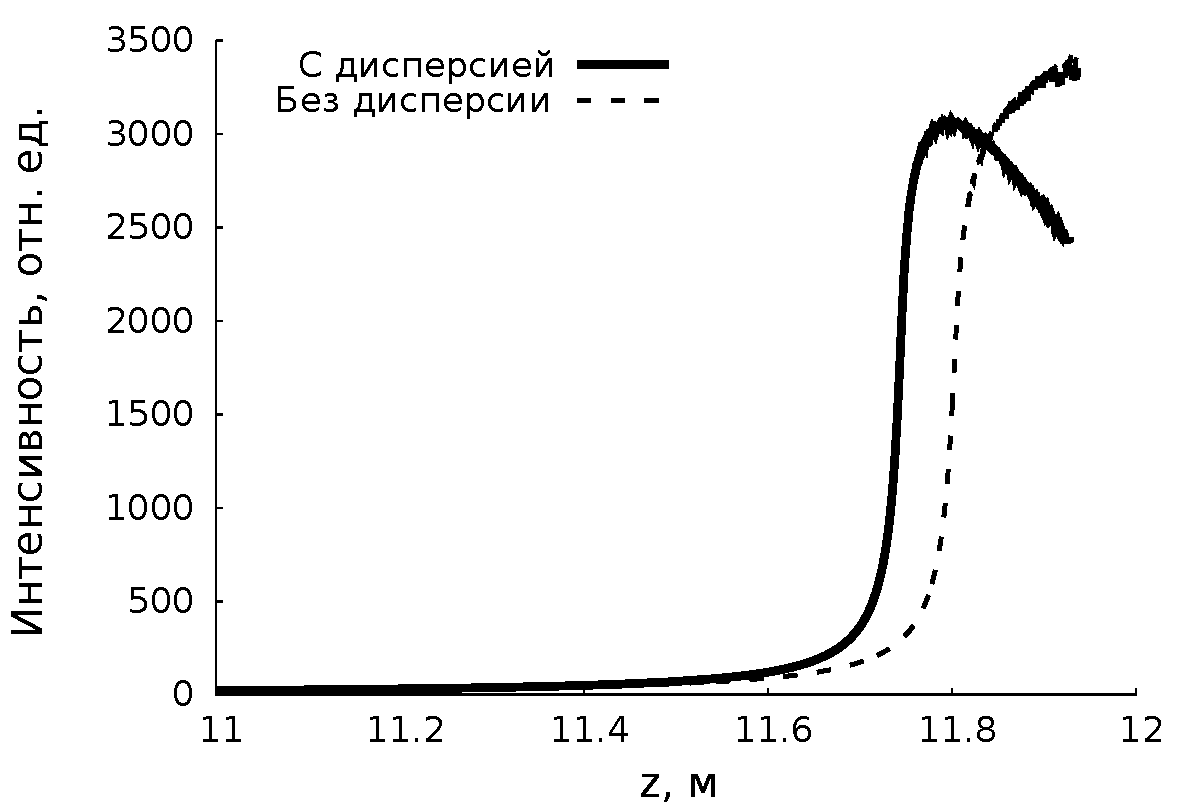
\includegraphics[width=0.95\linewidth]{pulses/noyes/intensity_cut}}
        \end{minipage}
        \\[1ex]
        \caption{Зависимость пиковой интенсивности в импульсе от расстояния распространения при~учёте и~без~учёта дисперсии второго порядка.
                 Параметры импульса: $\lambda = 800$~нм, $2r_0 = 2.5$~мм, $2\tau_0 = 750$~фс, $P = 1.5 P_{cr}$.}
        \label{fig:PulsesNoYesIntensity}
    \end{center}
\end{figure}

%%%%%%%%%%%%%%%%%%%%%%%%%%%%%%%%%%%%%%%%

Как видно из рис. \ref{fig:PulsesNoYesIntensity}, отсутствие дисперсии не сильно влияет на процесс префиламентации,
а проявляется только в небольшом сдвиге точки возникновения филамента. Однако, без учёта дисперсии интенсивность
продолжает нарастать слишком стремительно после прохождения этой точки, тогда как при учёте дисперсии
пиковая интенсивность достигает своего максимума и начинает уменьшаться. Это связано с~тем, что~дисперсия является
тем физическим механизмом, за счёт которого возможно ограничение временного сжатия импульса.
Так же, как при создании стабильного филамента возникает баланс между фокусирующим действием керровского эффекта
и дефокусирующего влияния возникающей плазмы, так и баланс между укорочением импульса за счёт поглощения энергии в хвосте импульса при взаимодействия его
с плазмой ограничено влиянием дисперсии. Таким образом, для ускорения расчётов возможно не учитывать дисперсию
на этапе префиламентации (а~точнее учитывать её с~помощью аналитических приближений), однако
при дальнейшем повышении интенсивности и возникновении плазмы пренебрегать дисперсией нельзя.
Для упрощения программы и получения более точных результатов все расчёты проводились
с учётом дисперсии второго порядка на всём пути распространения импульса.


\subsection{Характеристики филаментов на длине волны 800 нм}

Большая часть как теоретических, так и экспериментальных работ по филаментации выполняются с использованием излучения на длине волны 800 нм.
Таким образом для сравнения филаментации излучения на разных длинах волн удобно взять за основу именно эту длину волны.
Кроме того, это позволяет проверить корректность работы программы, сравнив получающиеся результаты с уже известными.
В качестве образца брались параметры импульса, указанные в кандидатской диссертации \cite{FedorovPhD2010}.

\begin{table}[H]
\begin{center}
\begin{tabular}{|c|c|c|c|c|c|c|}
\hline
  & $z_{fil}, \textrm{ м}$ & $I_{fil}, 10^{13} \textrm{ Вт}/\textrm{см}^2$ & $N_e^{fil}, 10^{16} \textrm{ см}^{-3}$ & $r_{fil}, \textrm{ мкм}$ & $r_{pl}, \textrm{ мкм}$ \\
\hline
а) & 2.48                  & 11.5                                          & 9.2                              & 43.4                     & 12.4                    \\
\hline
б) & 2.51                  & 12.7                                          & 9.4                              & 40.2                     & 9.3                     \\
\hline
\end{tabular}
\\[1ex]
\caption{Сравнение пиковых параметров филамента и плазменного канала с известными результатами при филаментации на длине волны 800 нм.
         В строке а) таблицы указаны уже известные результаты, в строке б) "--- вновь рассчитанные.
         Параметры импульса: $\tau_0 = 100 \textrm{ фс}$, $r_0 = 0.1 \textrm{ см}$, $P/P_{cr} = 3.93$, $L_{diff} = 7.85 \textrm{ м}$.}
\label{tab:PulsesCompareWithFedorov}
\end{center}
\end{table}

В таблице \ref{tab:PulsesCompareWithFedorov} приведены результаты сравнения пиковых характеристик филамента и~плазменого канала с полученными ранее.
Здесь $z_{fil}$ "--- положение максимума интенсивности по оси z, $I_{fil}$ "--- пиковая интенсивность в филаменте, $N_e^{fil}$ "--- пиковая концентрация свободных электронов, $r_{fil}$ "--- радиус филамента,
измеренный по уровню $e^{-1}$ от потока интенсивности (флюенса) в точке достижения пиковой концентрации электронов, $r_{pl}$ "--- радиус плазменного канала,
измеренный по уровню $e^{-1}$ от концентрации электронов после прохождения импульса. Количественное совпадение результатов подтверждает
возможность использования разработанной программы для исследования филаментации лазерных импульсов.

Для подготовки к сравнению процесса филаментации излучения на длине волны 800~нм и~10~мкм были выбраны другие параметры импульса.
На данный момент длительность импульсов $CO_2$-лазеров не достигает 100~фс, а~может быть не~меньше 500~фс по уровню $\frac{1}{2}$ от пиковой интенсивности \cite{PicosecondAmplifier2007},
поэтому было решено использовать для сравнения импульсы длительностью $2 \tau_0 = 750 \textrm{ фс}$.
При подборе параметров по возможности оставлялись неизменными большинство характеристик исходных импульсов.
Сравнение проводилось при одинаковом превышении критической мощности, \mbox{$P = 1.5P_{cr}$},
а для сохранения неизменной дифракционной длины при $\lambda = 800 \textrm{ нм}$ диаметр импульса брался равным $2 r_0 = 2.5 \textrm{ мм}$,
а для $\lambda = 10 \textrm{ мкм}$ "--- $2 r_0 = 8.8 \textrm{ мм}$. При этих параметрах дифракционная длина равнялась 12.2 м.

На графиках ниже приведены основные характеристики импульса в зависимости от пройденного расстояния в момент возникновения филамента.
Кроме наблюдения за~описанными выше пиковыми характеристиками филамента проводилось наблюдение за~радиусом и~длительностью пика интенсивности для контроля
того, чтобы он не становился меньше нескольких ячеек расчётной сетки. Для того, чтобы можно было говорить об адекватности результатов численного эксперимента,
необходимо было задавать шаг расчётной сетки таким, чтобы на всех шагах размер неоднородностей поля превышал шаг более, чем в два раза.
Для этого в центральной области сетки с~минимальным шагом он брался равным $h_r = 0.004$ и $h_t = 0.0005$.

%%%%%%%%%%%%%%%%%%%%%%%%%%%%%%%%%%%%%%%%

\begin{figure}[H]
    \begin{center}
        \begin{minipage}{\minipagewidthtwo}
            \center{\includegraphics[width=0.95\linewidth]{pulses/l800/intensity_z09}}
        \end{minipage}
        \hfill
        \begin{minipage}{\minipagewidthtwo}
            \center{\includegraphics[width=0.95\linewidth]{pulses/l800/plasma_z09}}
        \end{minipage}
        \\[1ex]
        \caption{Зависимости пиковой интенсивность и пиковой концентрации ионов от пройденного расстояния при филаментации излучения на длине волны 800 нм.}
        \label{fig:Pulses800INe}
    \end{center}
\end{figure}

%%%%%%%%%%%%%%%%%%%%%%%%%%%%%%%%%%%%%%%%

%%%%%%%%%%%%%%%%%%%%%%%%%%%%%%%%%%%%%%%%

\begin{figure}[H]
    \begin{center}
        \begin{minipage}{\minipagewidthtwo}
            \center{\includegraphics[width=0.95\linewidth]{pulses/l800/r_fil_z09}}
        \end{minipage}
        \hfill
        \begin{minipage}{\minipagewidthtwo}
            \center{\includegraphics[width=0.95\linewidth]{pulses/l800/r_pl_z09}}
        \end{minipage}
        \\[1ex]
        \caption{Зависимости радиуса филамента и плазменного канала от пройденного расстояния при~филаментации излучения на длине волны 800 нм.}
        \label{fig:Pulses800RFilPl}
    \end{center}
\end{figure}

%%%%%%%%%%%%%%%%%%%%%%%%%%%%%%%%%%%%%%%%

Как видно из рис. \ref{fig:Pulses800INe}, длина филамента по уровню $e^{-1}$ по интенсивности заведомо больше 50~см.
Если же рассчитать дифракционную длину для импульса с радиусом 50~мкм (это радиус образовавшегося филамента,
что видно на рис. \ref{fig:Pulses800RFilPl}), то мы получим:

\begin{equation}
L_{diff}^{fil} = \frac{2\pi}{800 \cdot 10^{-9}} \cdot (50 \cdot 10^{-6})^2 \textrm{ м} = 1.96 \textrm{ см}.
\end{equation}

\noindent Таким образом, можно говорить об образовании филамента, а не об обычном случае острой фокусировки пучка.

%%%%%%%%%%%%%%%%%%%%%%%%%%%%%%%%%%%%%%%%

\begin{figure}[H]
    \begin{center}
        \begin{minipage}{\minipagewidththree}
            \center{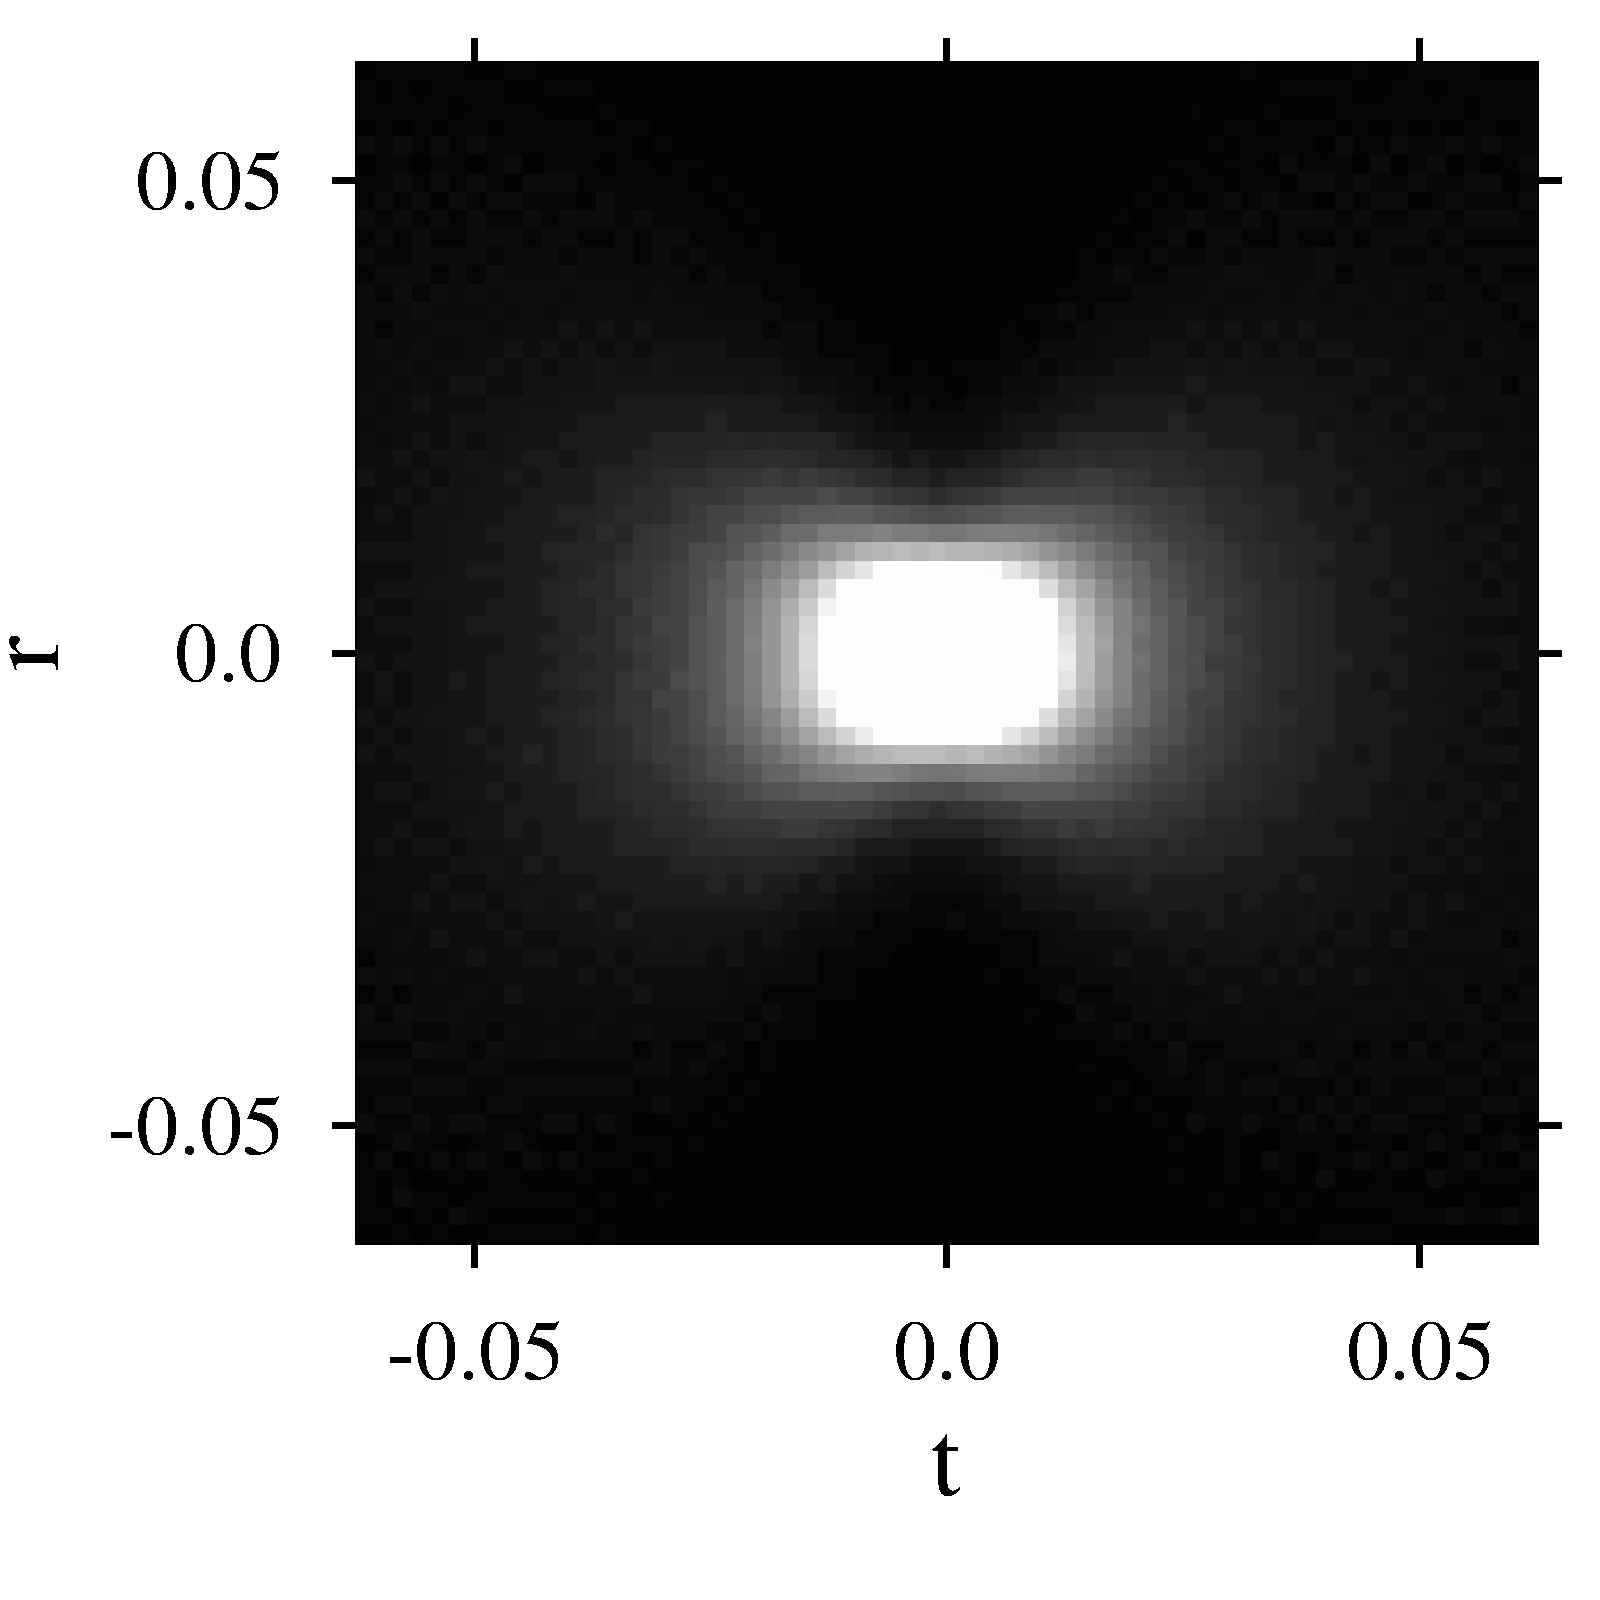
\includegraphics[width=0.95\linewidth]{pulses/l800_images/out00600_all_norm} \\[0.1ex]
            \footnotesize{$z = 0.958$}}
        \end{minipage}
        \hfill
        \begin{minipage}{\minipagewidththree}
            \center{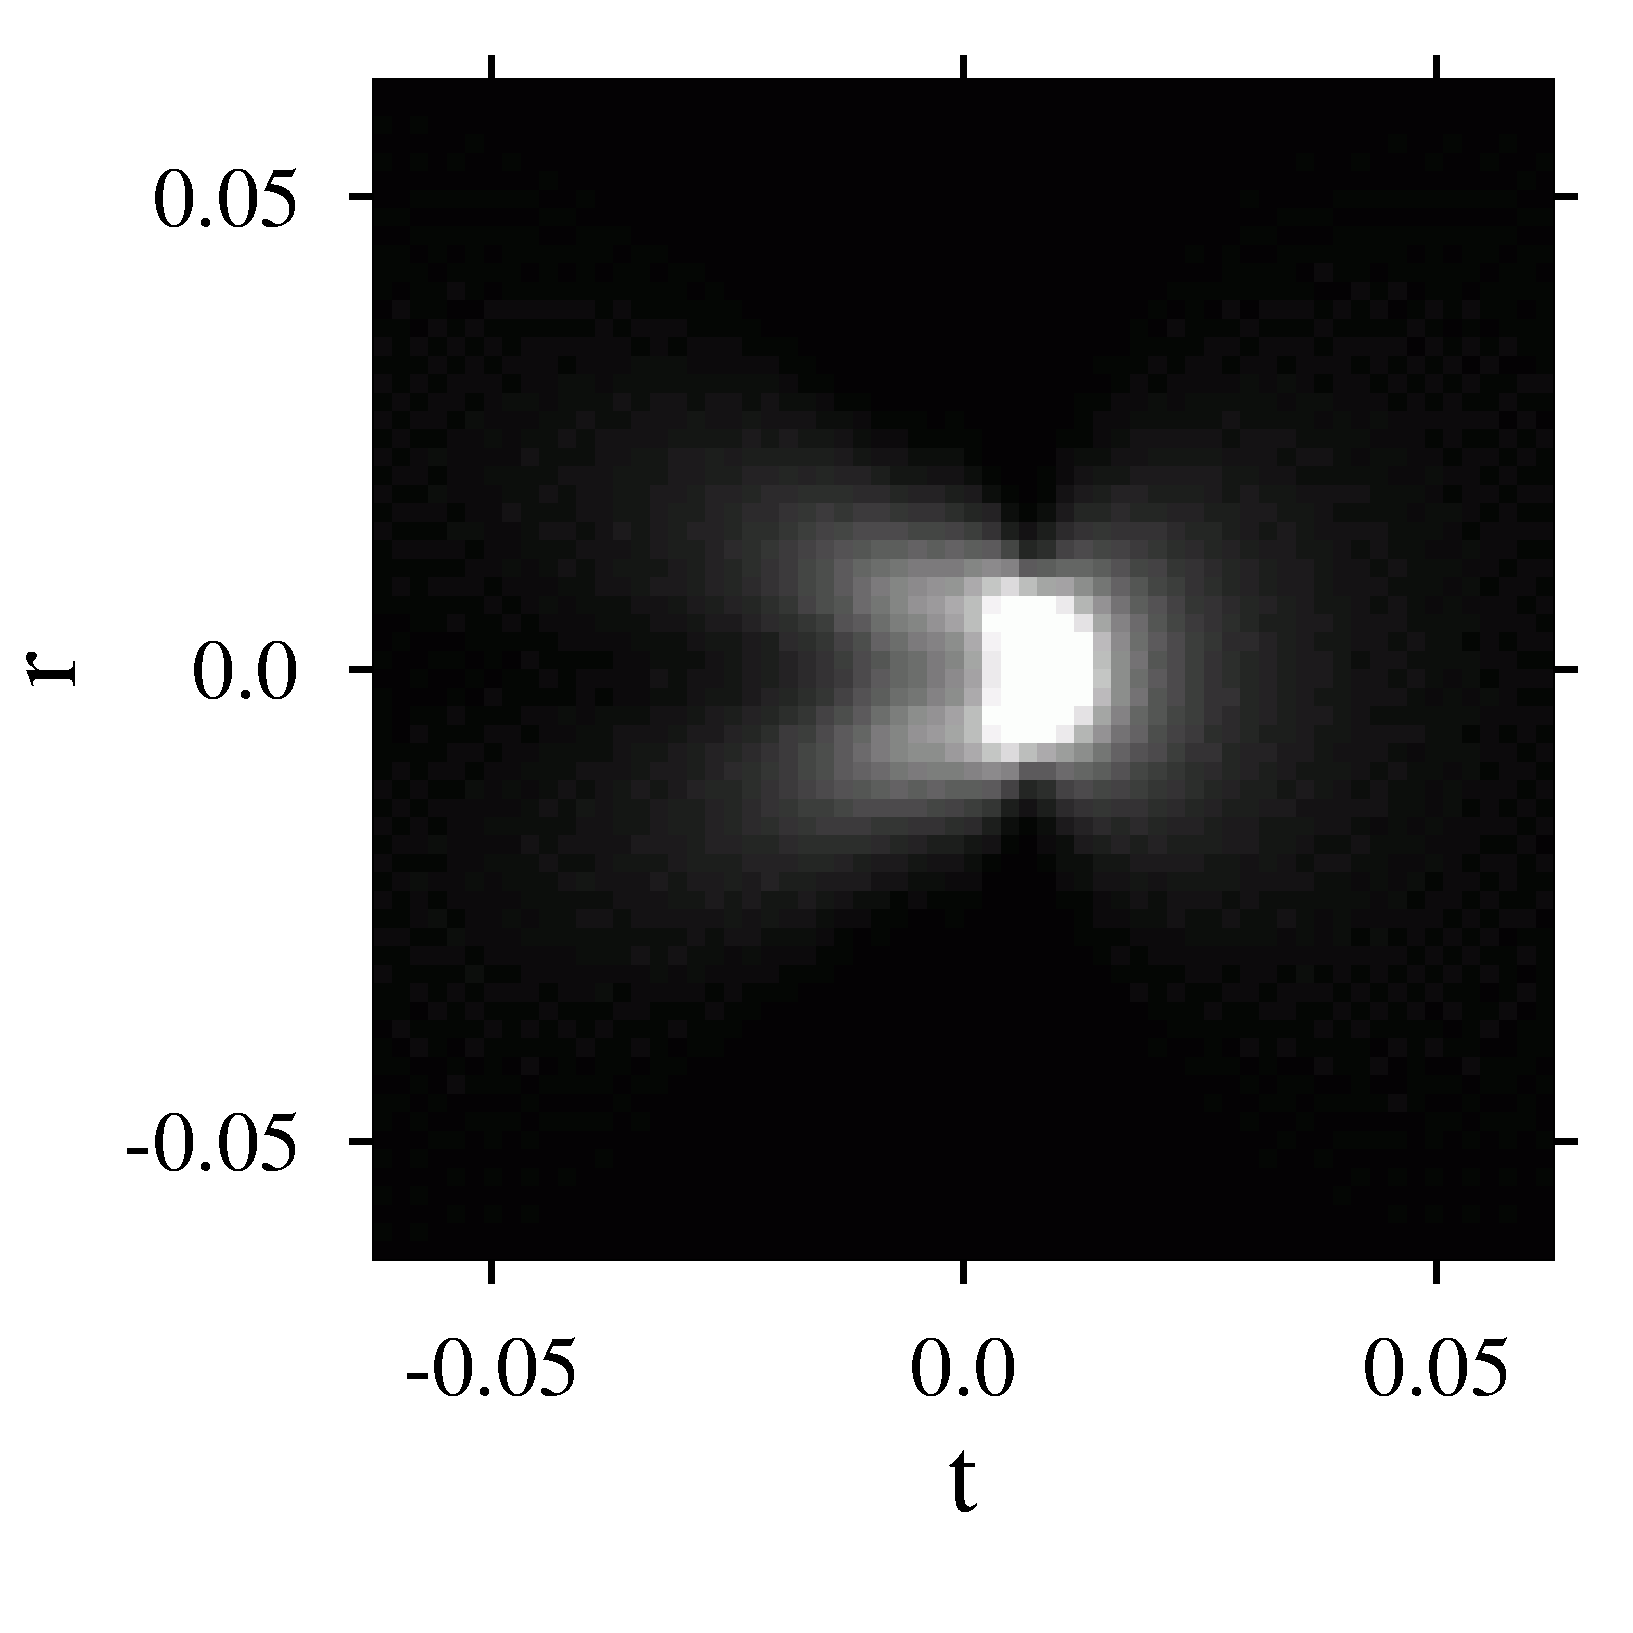
\includegraphics[width=0.95\linewidth]{pulses/l800_images/out00800_all_norm} \\[0.1ex]
            \footnotesize{$z = 0.9599$}}
        \end{minipage}
        \hfill
        \begin{minipage}{\minipagewidththree}
            \center{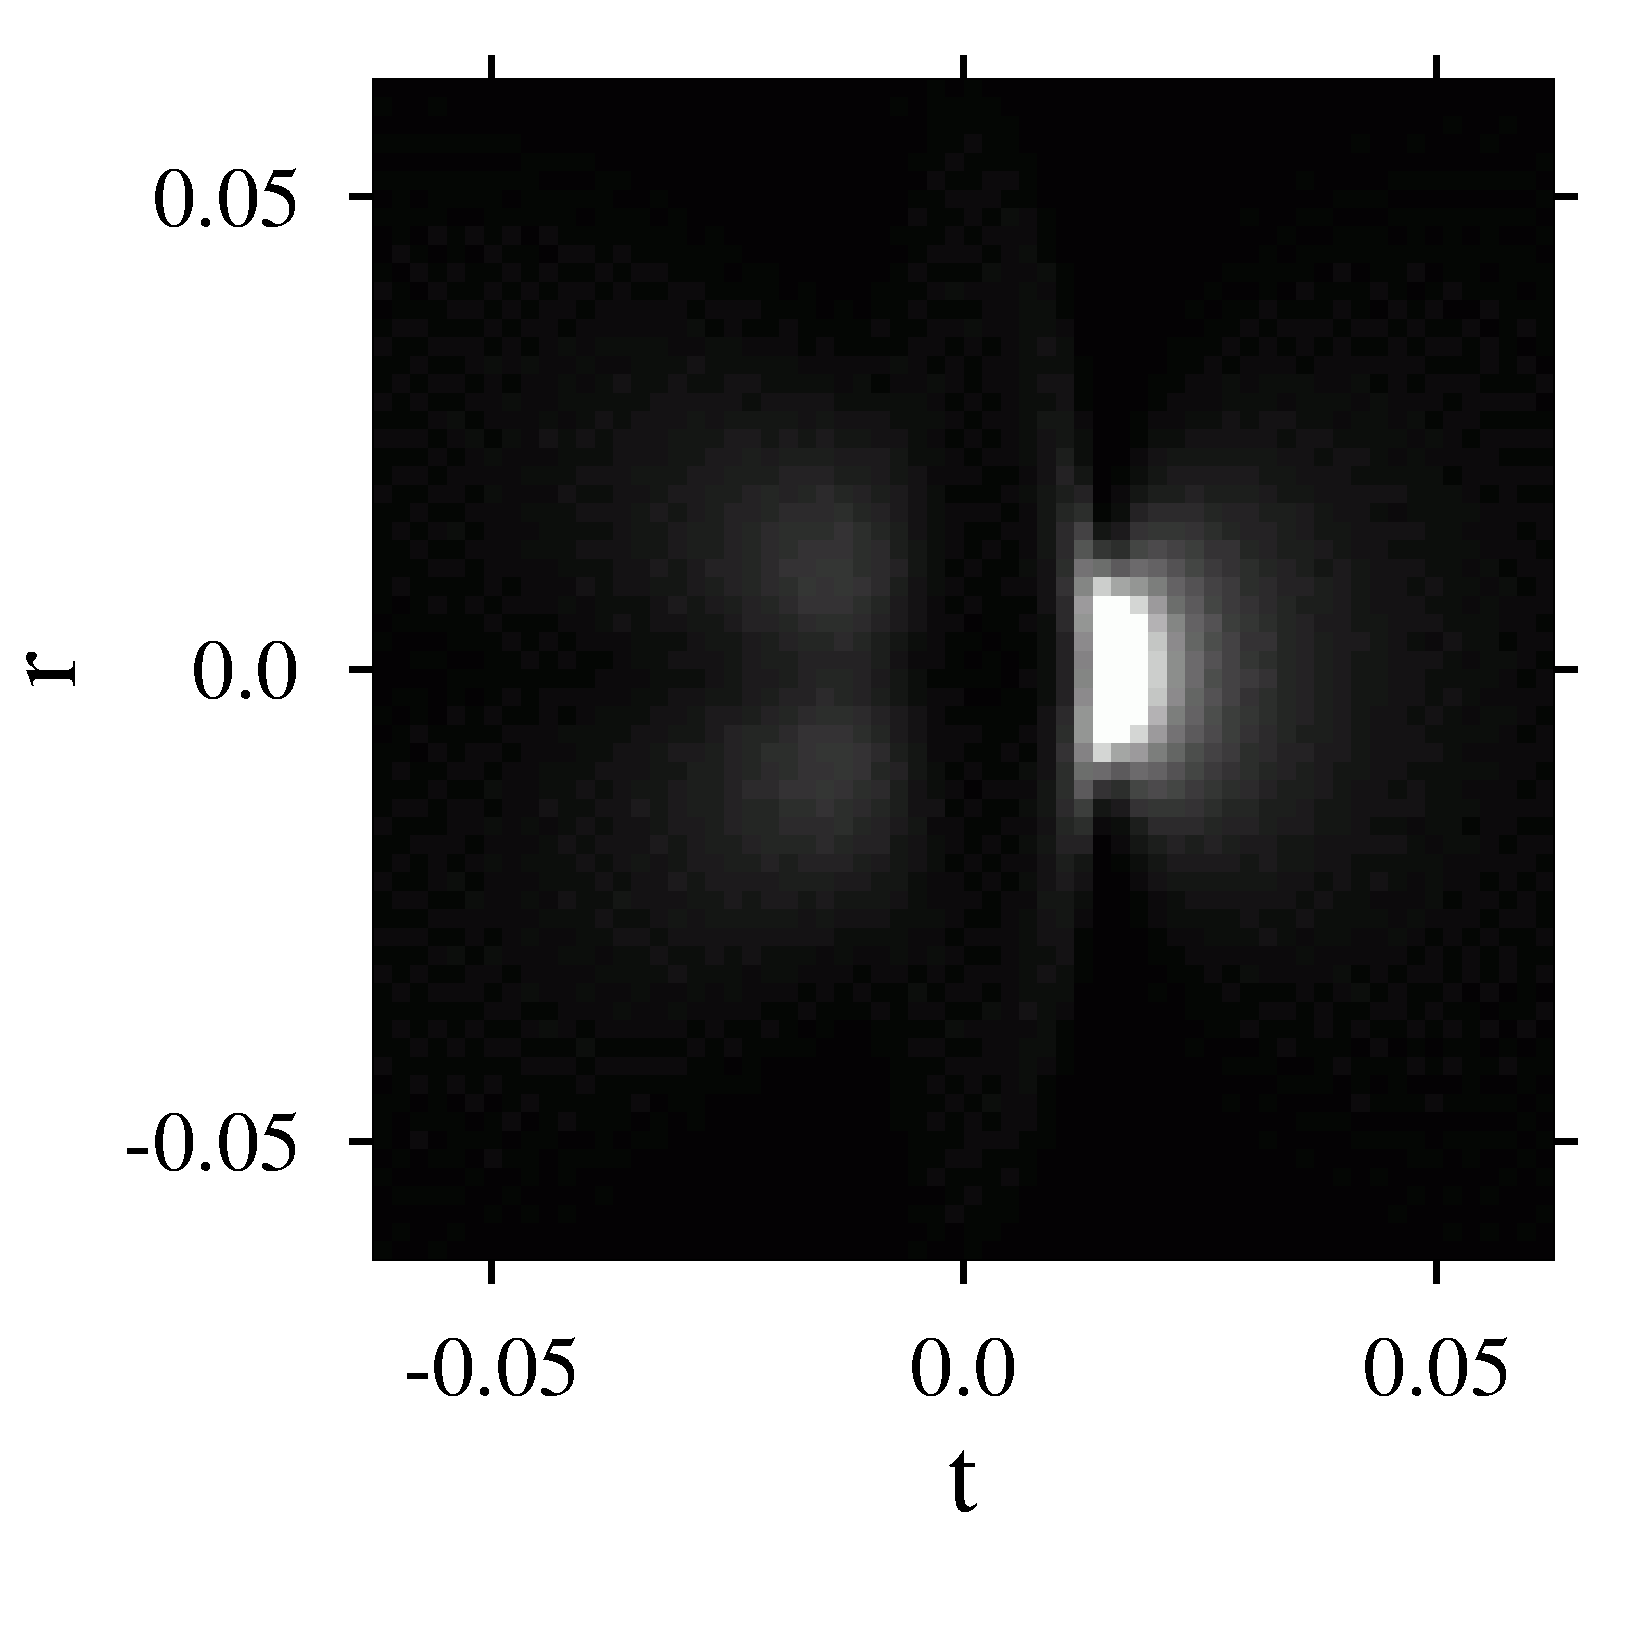
\includegraphics[width=0.95\linewidth]{pulses/l800_images/out01200_all_norm} \\[0.1ex]
            \footnotesize{$z = 0.9627$}}
        \end{minipage}
        \\[1ex]
        \caption{Характерные распределения интенсивности в импульсе в процессе филаментации излучения на длине волны 800 нм.
                 Переменные обезразмерены на начальную длительность и радиус импульса, соответственно.}
        \label{fig:PulsesRTBW}
    \end{center}
\end{figure}

%%%%%%%%%%%%%%%%%%%%%%%%%%%%%%%%%%%%%%%%

Характерные распределения интенсивности в импульсе приведены на рис. \ref{fig:PulsesRTBW}. На~нём можно наблюдать первоначальное сжатие центральной части импульса
под действием керровской фокусировки и дальнейшее изменение пространственно"=временной формы за счёт взаимодействия с индуцированной плазмой.
На последней иллюстрации рис. \ref{fig:PulsesRTBW} видно образование области повышенной интенсивности позади основного пика интенсивности импульса.
В дальнейшем может произойти рефокусировка этой области и образование второго субимпульса.
К сожалению, используемая модель не позволяет провести расчёт до этого момента, так как не учитывается дисперсия высших порядков
и влияние операторов $\frac{i}{\omega}\frac{\partial }{\partial t}$, из-за чего задний фронт импульса становится слишком крутым
и перестаёт разрешаться на сетке с любым самым малым шагом.


\subsection{Филаментация импульсов на длине волны 10 мкм}

Было проведено сравнение процесса филаментации и характеристик филамента \\ при~длине волны 800~нм и 10~мкм.
Импульс излучения на длине волны 10~мкм брался со~следующими параметрами: $2 \tau_0 = 750 \textrm{ фс}$, $P = 1.5P_{cr}$, $2 r_0 = 8.8 \textrm{ мм}$.
Как было сказано выше, другой радиус импульса был взят для того, чтобы дифракционный масштаб остался неизменным.
Были получены пиковые величины интенсивности, концентрации электронов, радиусы филамента и плазменного канала как функции расстояния распространения.

%%%%%%%%%%%%%%%%%%%%%%%%%%%%%%%%%%%%%%%%

\begin{figure}[H]
    \begin{center}
        \begin{minipage}{\minipagewidthtwo}
            \center{\includegraphics[width=0.95\linewidth]{pulses/l10000/intensity_z09}}
        \end{minipage}
        \hfill
        \begin{minipage}{\minipagewidthtwo}
            \center{\includegraphics[width=0.95\linewidth]{pulses/l10000/plasma_z09}}
        \end{minipage}
        \\[1ex]
        \caption{Зависимости пиковой интенсивность и пиковой концентрации ионов от пройденного расстояния~при филаментации излучения на длине волны 10 мкм.}
        \label{fig:Pulses10000INe}
    \end{center}
\end{figure}

%%%%%%%%%%%%%%%%%%%%%%%%%%%%%%%%%%%%%%%%

%%%%%%%%%%%%%%%%%%%%%%%%%%%%%%%%%%%%%%%%

\begin{figure}[H]
    \begin{center}
        \begin{minipage}{\minipagewidthtwo}
            \center{\includegraphics[width=0.95\linewidth]{pulses/l10000/r_fil_z09}}
        \end{minipage}
        \hfill
        \begin{minipage}{\minipagewidthtwo}
            \center{\includegraphics[width=0.95\linewidth]{pulses/l10000/r_pl_z09}}
        \end{minipage}
        \\[1ex]
        \caption{Зависимости радиуса филамента и плазменного канала от пройденного расстояния при~филаментации излучения на длине волны 10 мкм.}
        \label{fig:Pulses10000RFilPl}
    \end{center}
\end{figure}

%%%%%%%%%%%%%%%%%%%%%%%%%%%%%%%%%%%%%%%%

Как видно из рис. \ref{fig:Pulses10000INe}-\ref{fig:Pulses10000RFilPl}, с увеличением длины волны увеличиваются диаметры филамента
и плазменного канала, тогда как концентрация ионов в плазме уменьшается. Это можно качественно объяснить следующим образом: в момент, когда прекращается рост интенсивности
нелинейные добавки к показателю преломления, вызванные керровской нелинейностью и плазменной дефокусировкой, должны скомпенсировать друг друга:

\begin{equation}
\Delta n_k(z_{fil}) = \frac{1}{2}n_2 I_{fil} = \frac{\omega_p^2}{2 n_0 \omega_0^2} = -\Delta n_pl(z_{fil})
\end{equation}

Если считать, что $n_2$ и $I_{fil}$ не сильно зависят от длины волны, а мощность излучения в филаменте равна ровно одной критической мощности,
можно получить следующие оценки \cite{FedorovKandidovDifferentWavelengths2008}:

\begin{align}\label{PulsesAnaliticEq}
N_e^{fil}(\lambda) & \sim \frac{1}{\lambda^2} \\
r_{fil} & \sim \lambda \\
r_{pl} & \sim \lambda
\end{align}

По данным \cite{FedorovKandidovDifferentWavelengths2008}, численные результаты для филаментации на длинах волн 248--1240~нм хорошо описываются этими зависимостями.
Однако, как можно убедиться по~рис.~\ref{fig:PulsesAnalitic}, полученные в настоящей работе характеристики филаментации на длине волны 10 мкм этими зависимостями описываются
не очень точно. На графиках приведены аппроксимации по формулам (\ref{PulsesAnaliticEq}),
построенные по ранее известным данным \cite{FedorovPhD2010} и~добавлена точка для вновь полученных параметров
при филаментации излучения на~длине волны 10~мкм.

%%%%%%%%%%%%%%%%%%%%%%%%%%%%%%%%%%%%%%%%

\begin{figure}[H]
    \begin{center}
        \begin{minipage}{\minipagewidthtwo}
            \center{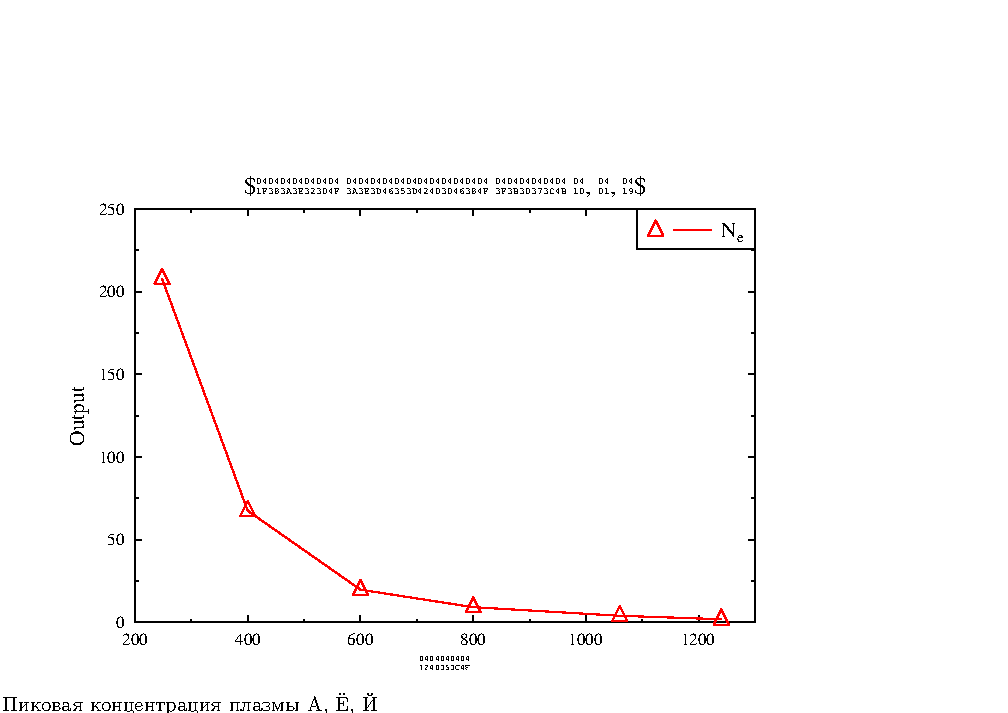
\includegraphics[width=0.95\linewidth]{pulses/comparison/plasma}}
        \end{minipage}
        \hfill
        \begin{minipage}{\minipagewidthtwo}
            \center{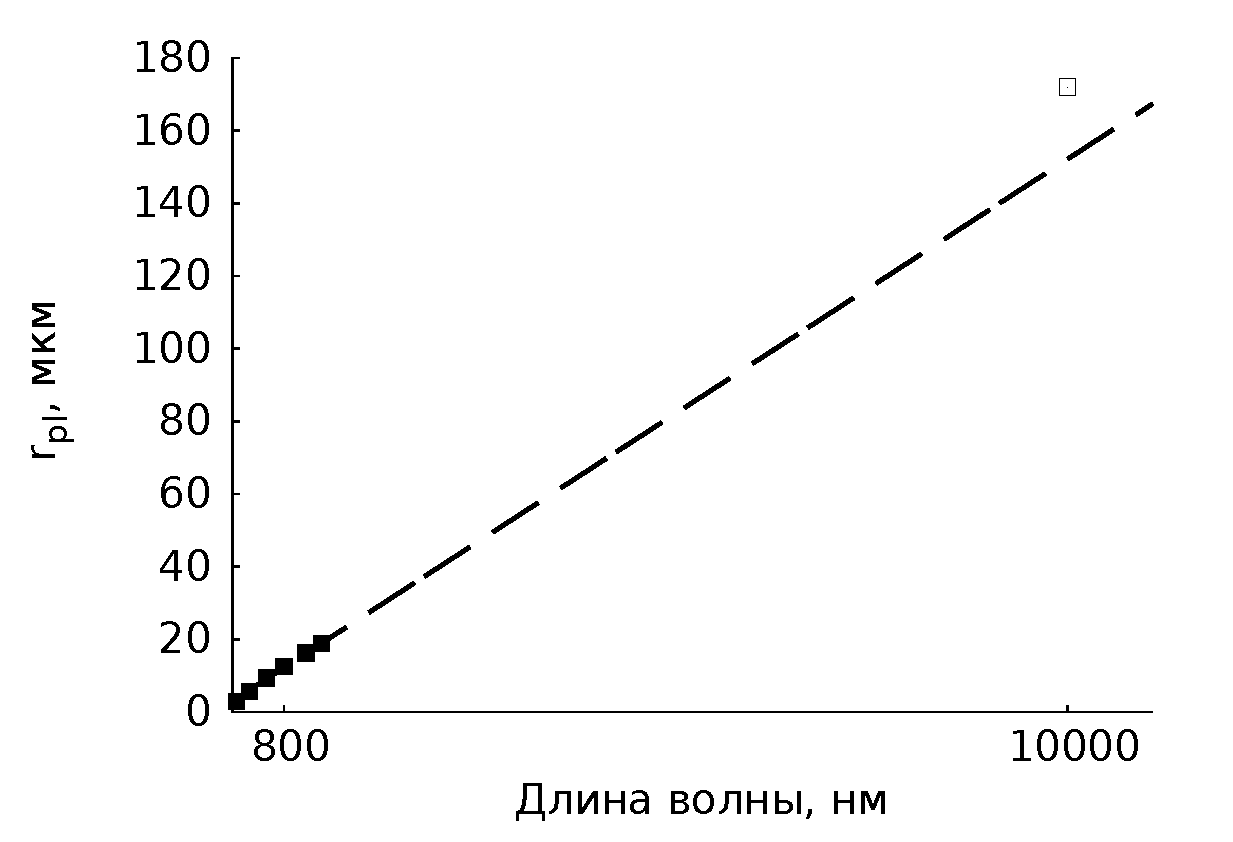
\includegraphics[width=0.95\linewidth]{pulses/comparison/r_pl}}
        \end{minipage}
        \\[1ex]
        \caption{Сравнение полученных характеристик плазменного канала филамента на длине волны 10~мкм с уже известными данными по длинам волн 248--1240~нм.
                 На графиках заполненными точками отмечены данные из \cite{FedorovPhD2010}, кривые аппроксимируют их по формулам (\ref{PulsesAnaliticEq}), а пустая точнка обозначает полученные численные результаты.}
        \label{fig:PulsesAnalitic}
    \end{center}
\end{figure}

%%%%%%%%%%%%%%%%%%%%%%%%%%%%%%%%%%%%%%%%

Также при изменении длины волны меняется характер плазмообразования: если на~длине волны 800~нм кислородных ионов было в среднем в два раза больше, чем азотных, то при филаментации
излучения на длине волны 10 мкм кислородные ионы преобладают. Для сравнения основные характеристики филамента и плазменного канала при~одинаковой дифракционной длине, длительности импульса
и одинаковым превышением критическорй мощности приведены в таблице \ref{tab:PulsesCompare800vs10000}.

\begin{table}[H]
\begin{center}
\begin{tabular}{|r|c|c|c|c|c|c|}
\hline
$\lambda$, нм & $r_0$, см & $z_{fil}$, м & $I_{fil}, \textrm{ Вт}/\textrm{см}^2$ & $N_e^{fil} (N_e^{O} + N_e^{N}), 10^{16} \textrm{ см}^{-3}$ & $r_{fil}, \textrm{ мкм}$   & $r_{pl}, \textrm{ мкм}$ \\
\hline
800            & 0.125     & 11.77        & $8.91 \cdot 10^{13}$                   & 4.4 (3.3 + 1.1)                                             & 38.2 (68.4)                 & 8.8 (8.7)                \\
\hline
10000          & 0.442     & 11.52        & $4.12 \cdot 10^{13}$                   & $\approx$ 0.01 (0.01 + 0.0005)                             & 839 (1213)                  & 198 (205)                 \\
\hline
\end{tabular}
\\[1ex]
\caption{Сравнение расстояния филаментации, пиковой интенсивности, пиковой концентраций плазмы,
         и радиусов филамента и плазменного канала при филаментации излучения на~длинах волн 800~нм и~10~мкм.
         Для радиусов также в скобках указаны средние от точки пиковой интенсивности до~точки падения интенсивности в $e^{-1}$ раз.
         Параметры импульса: $\tau_0 = 375 \textrm{ фс}$, $P/P_{cr} = 1.5$, $L_{diff} = 12.17 \textrm{ м}$.}
\label{tab:PulsesCompare800vs10000}
\end{center}
\end{table}

%%%%%%%%%%%%%%%%%%%%%%%%%%%%%%%%%%%%%%%%

\begin{figure}[H]
    \begin{center}
        \begin{minipage}{\minipagewidthtwo}
            \center{\includegraphics[width=0.95\linewidth]{pulses/l800/energy_log_z09}} \\
            \footnotesize{(а)}
        \end{minipage}
        \begin{minipage}{\minipagewidthtwo}
            \center{\includegraphics[width=0.95\linewidth]{pulses/l10000/energy_log_z09}} \\
            \footnotesize{(б)}
        \end{minipage}
        \\[1ex]
        \caption{Зависимости полной энергии импульса и потерь на поглощение от пройденного расстояния при~филаментации излучения на длине волны 800~нм~(а) и~10~мкм~(б).}
        \label{fig:PulsesEnergy}
    \end{center}
\end{figure}

%%%%%%%%%%%%%%%%%%%%%%%%%%%%%%%%%%%%%%%%

Отдельно хочется отметить, что, как показали проведённые расчёты, учёт поглощения излучения генерируемой плазмой не является обязательным на этом этапе расчёта.
Поглощённая энергия на несколько порядков меньше, чем энергия, ушедшая из расчётной области, и в сумме они также практически не влияют на полную энергию импульса.


\subsection{Выводы}

Для обоснования необходимости рассмотрения нестационарной задачи было показано влияние
дисперсии второго порядка на распространение филамента до точки достижения первого максимума интенсивности.
В ходе расчётов также было получено, что~для~исследования распространения сформировавшегося филамента
необходимо учитывать дисперсию высших порядков и волновую нестационарность.

Проведены тестовые эксперименты, показывающие высокую точность используемых алгоритмов на этапе префиламентации и до достижения пиковой интенсивности.
Проведено сравнение получающихся результатов для длины волны 800~нм с~известными из~литературы и~показано их~количественное совпадение.

Для двух импульсов с одинаковыми длительностями, дифракционной длиной и превышением пиковой мощности над критической
при длинах волн 800~нм и~10~мкм проведено сравнение характеристик возникающего филамента и плазменного канала.
Показано, что при увеличении длины волны излучения диаметр филамента и плазменного канала увеличиваются,
тогда как концентрация плазмы уменьшается.
Это поведение предсказывается аналитическими зависимостями и экспериментальными данными,
полученными для диапазона длин волн 248--1240~нм,
что не позволяют получить количественного соответствия теоретического значения
с полученным в эксперименте для~длины волны 10~мкм.
Показано, что при изменении длины волны излучения увеличивается процентное содержание ионов кислорода в образующейся плазме.

